% Provenance (never printed): see sources/outline_sources.md (Year 1: field
% notebook, compass-clinometer, hand lens, sampling, polarising microscope and
% thin sections, safety). The readings of the Varden east limb are simulated
% in figdata/bachelor-1/attitude_stats.py (seed 83, errors of 3 degrees);
% problem values in the Book 3 scratch calculator calc/ch06.py.
\chapter{Veldwerk- en laboratoriummethoden I}\label{ch:b1:field-lab-methods-1}

Een geoloog die de Varden Hills in kaart brengt, draagt weinig mee: een notitieboekje, een potlood, een
satellietontvanger, een kompas-kliseometer, een handlens en een paar monsterzakjes. Daarmee bepaalt zij waar
zij staat, meet zij de oriëntatie van de lagen, benoemt zij de gesteenten en brengt zij de monsters terug die
het laboratorium zal zagen, malen en onder een microscoop bekijken. Elk getal van de voorgaande hoofdstukken ---
een oriëntatie op een kaart, een helling in een doorsnede --- begon als zo'n aflezing, met haar eigen fout.
Dit hoofdstuk beschrijft hoe professionals deze waarnemingen doen, en hoe herhaalde aflezingen worden gemiddeld
en hun spreiding in een onzekerheid wordt omgezet. Het eindigt met een veldseizoen van aflezingen op de oostflank
van de \omterm{def:b1:geological-maps:fold}{antiklinaal} van Varden.

\begin{recall}
De oriëntatie van een vlak wordt geschreven als \omterm{def:b1:geological-maps:attitude}{hellingrichting}/helling, bijvoorbeeld $081/12$, of als een \omterm{def:b1:geological-maps:attitude}{strijk}
volgens de rechterhandregel met een helling (\cref{ch:b1:geological-maps}). De magnetische declinatie is de hoek
tussen het geografische noorden en de \omterm{def:b1:field-lab-methods-1:trend-plunge}{richting} waarin een kompasnaald wijst (natuurkunde, klas 11). Mineralen
worden in de hand herkend aan hun glans, splijting, hardheid en kleur (Boek 2, klas 11). Het gemiddelde en de
standaardafwijking van een reeks getallen vatten hun midden en hun spreiding samen (wiskunde).
\end{recall}

\section{Het veldboek en de kaart}

\begin{definition}[Veldstation, veldboek]\label{def:b1:field-lab-methods-1:station}
Een \emph{veldstation}\index{veldstation} is een genummerde plaats waar een geoloog waarnemingen doet en
registreert: haar positie, de gesteenten die zij ziet, hun oriëntatie en de genomen monsters. Het
\emph{veldboek}\index{veldboek} is het ingebonden verslag van de stations, in de volgorde waarin ze zijn bezocht,
met hun nummers, schetsen en metingen, ter plaatse geschreven.
\end{definition}

Het notitieboekje is de primaire registratie: wat niet op het station is opgeschreven, gaat verloren, en een kaart
die 's avonds is getekend, is niet beter dan de aantekeningen eronder. Elk station heeft een nummer dat op de veldkaart,
in het notitieboekje en op elk monsterzakje dat er is genomen verschijnt. Een schets toont wat een lijst van getallen
niet kan tonen --- hoe twee eenheden samenkomen, welke kant de jongere lagen op liggen, waar een meting op een geplooid
oppervlak is gedaan --- en legt schaal en oriëntatie vast. Feiten en interpretaties worden uit elkaar gehouden:
``kalksteen op schalie, scherp contact'' is een waarneming; ``\omterm{def:b1:cross-sections:unconformity}{discordantie}'' is een gevolgtrekking, en wordt als
zodanig geschreven.

\begin{inthefield}[Een dag kaarteren]
% ledger: gps:smartphone-accuracy, gps:high-end
\begin{minipage}[t]{0.58\linewidth}\vspace{0pt}
Een kaarterende geoloog plant een traverse dwars op de \omterm{def:b1:geological-maps:attitude}{strijk}, zodat zij elke eenheid achtereenvolgens bereikt, en
stopt waar een contact, een verandering van gesteente of een meetbaar oppervlak verschijnt. Op elk station schrijft
zij het stationsnummer en de positie, schetst zij wat zij ziet, meet zij oriëntaties en noteert zij de monsters.
De posities komen van een satellietontvanger: een gewone ontvanger, zoals die van een smartphone, is onder open hemel
doorgaans nauwkeurig tot ongeveer \qty{4.9}{m}, slechter nabij rotswanden en bomen, terwijl meetontvangers die twee
frequenties gebruiken of correctiediensten gebruiken, enkele centimeters halen. Op een kaartschaal van 1:10\,000 is
\qty{4.9}{m} een half millimeter: een gewone ontvanger is goed genoeg voor de kartering, maar niet om de trage beweging
van de grond te meten (\cref{ch:b1:plate-kinematics}).
\end{minipage}\hfill
\begin{minipage}[t]{0.39\linewidth}\vspace{0pt}
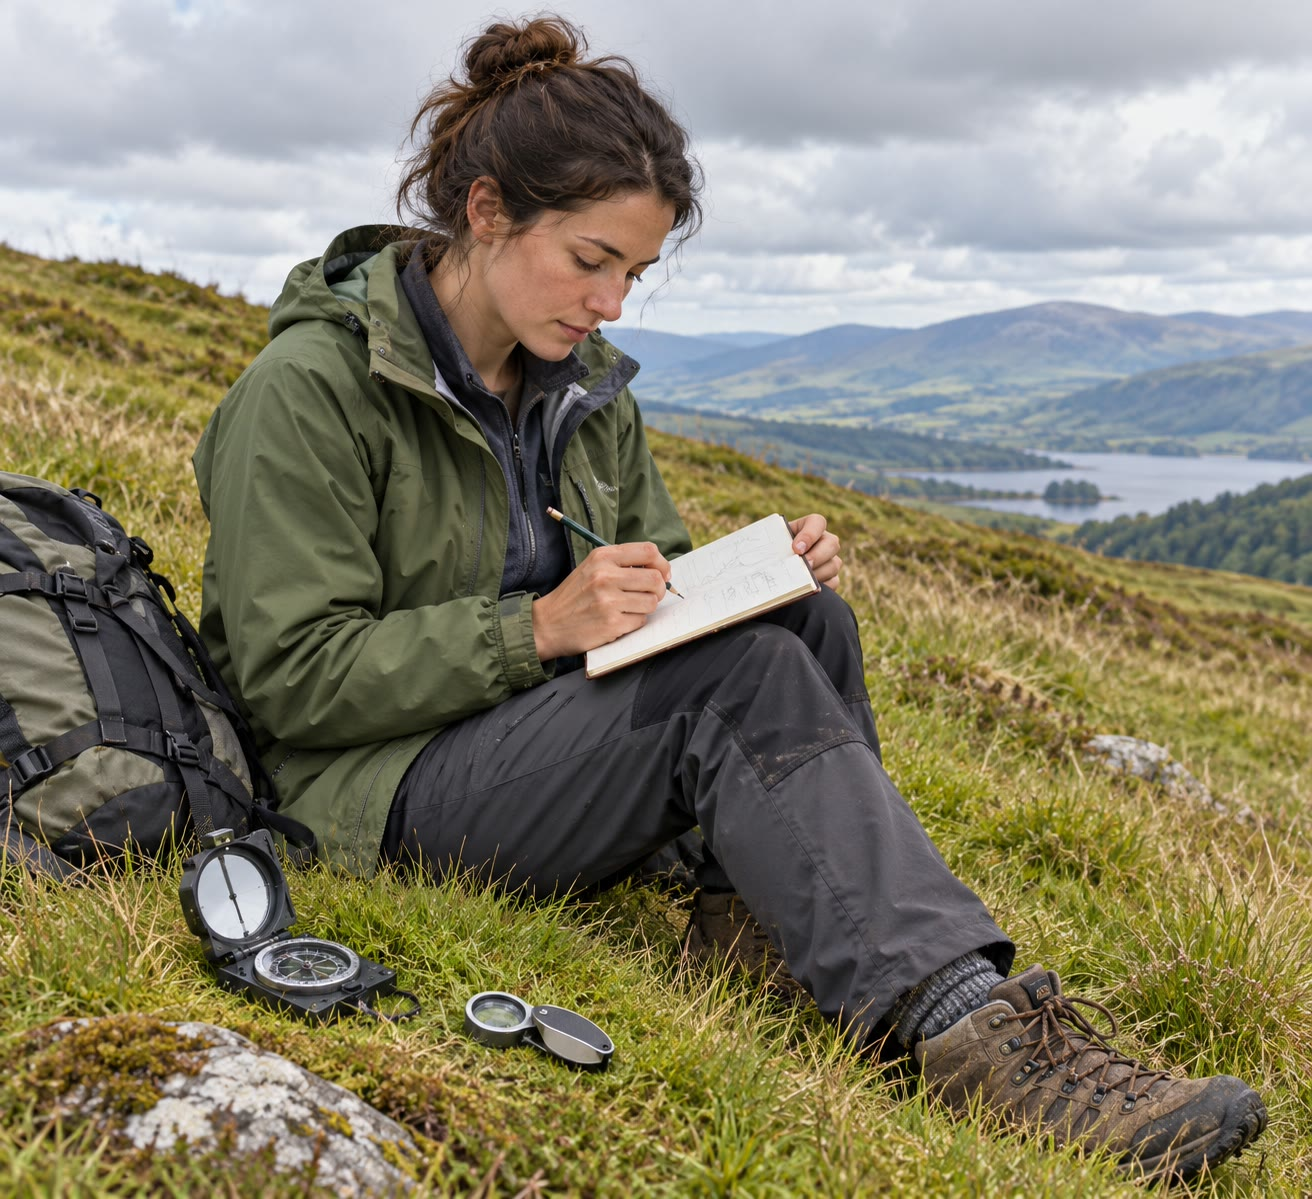
\includegraphics[width=\linewidth]{images/book3/ai/b1-field-notebook.jpg}
\end{minipage}
\end{inthefield}

\section{Oriëntaties meten}

De oriëntatie van een vlak --- een laag, een breuk, een spleet --- wordt met een kompas-kliseometer gemeten: een magnetisch
kompas om \omterm{def:b1:spherical-astronomy:horizontal}{azimuten} af te lezen, en een slinger of waterpas om hoeken ten opzichte van de horizontale af te lezen. Haar rand
wordt langs de \omterm{def:b1:geological-maps:attitude}{strijk} van het oppervlak gelegd om de \omterm{def:b1:geological-maps:attitude}{strijk} af te lezen, of het instrument wordt op het oppervlak gezet langs
zijn steilste lijn om de helling af te lezen en, uit het \omterm{def:b1:spherical-astronomy:horizontal}{azimut} van die lijn, de \omterm{def:b1:geological-maps:attitude}{hellingrichting}.

\begin{omfigure}
\begin{tikzpicture}[font=\scriptsize]
% (a) plan view
\begin{scope}
\fill[icsJurassic!25] (0,0) -- (3.6,0.5) -- (3.9,2.9) -- (0.3,2.4) -- cycle;
\draw (0,0) -- (3.6,0.5) -- (3.9,2.9) -- (0.3,2.4) -- cycle;
\draw[omDef, thick] (0.4,1.55) -- (3.5,1.98);
\node[omDef, above, rotate=8, fill=icsJurassic!25, inner sep=1pt] at (0.95,1.65) {strijklijn};
% compass box laid along the strike line
\begin{scope}[shift={(2.5,1.84)}, rotate=8]
\draw[fill=white] (-0.6,0) rectangle (0.6,0.32);
\draw (0,0.16) circle (0.12);
\end{scope}
\draw[omThm, thick, -{Stealth[length=2mm]}] (1.6,1.71) -- (1.75,0.62);
\node[omThm, right, fill=icsJurassic!25, inner sep=1pt] at (1.78,0.85) {hellingrichting};
\node[below, align=center] at (1.95,-0.15) {(a) bovenaanzicht: de rand van\\ het kompas langs de strijk};
\draw[->] (4.3,1.6) -- (4.3,2.4) node[above] {N};
\end{scope}
% (b) side view, vertical section along the dip direction
\begin{scope}[xshift=5.8cm]
\fill[icsJurassic!25] (0,1.6) -- (3.6,0.2) -- (3.6,-0.3) -- (0,-0.3) -- cycle;
\draw[thick] (0,1.6) -- (3.6,0.2);
% clinometer resting on the surface
\begin{scope}[shift={(2.5,0.6278)}, rotate=-21.25]
\draw[fill=white] (-0.75,0) rectangle (0.75,0.3);
\draw (0,0.15) circle (0.11);
\draw[black!70] (0,0.15) -- ++(-68.75:0.11);
\end{scope}
% dip angle at the lower end of the surface
\coordinate (P) at (0.7,1.3278);
\draw[black!60] (P) -- ++(1.6,0) node[right] {horizontaal};
\draw[omThm] ($(P)+(1.1,0)$) arc[start angle=0, end angle=-21.25, radius=1.1];
\node[omThm] at ($(P)+(0.9,-0.15)$) {$\delta$};
\node[below, align=center] at (1.8,-0.35) {(b) doorsnede langs de hellingrichting:\\ de kliseometer op de steilste lijn};
\end{scope}
\end{tikzpicture}

{\small Het meten van een oriëntatie (schematisch). (a) De rand van het kompas, horizontaal op de laag gelegd, geeft de \omterm{def:b1:geological-maps:attitude}{strijk};
de \omterm{def:b1:geological-maps:attitude}{hellingrichting} staat er loodrecht op, de laag af. (b) Op zijn kant langs de steilste lijn gezet, geeft de kliseometer de
helling $\delta$.}
\end{omfigure}

Een lijn --- een \omterm{def:b1:geological-maps:fold}{plooias}, een kras op een breukvlak, de lange as van keien --- heeft een oriëntatie van zichzelf.

\begin{definition}[Richting en duik van een lijn]\label{def:b1:field-lab-methods-1:trend-plunge}
De \emph{richting}\index{richting (van een lijn)} van een lijn is het \omterm{def:b1:spherical-astronomy:horizontal}{azimut} van haar horizontale projectie, gemeten
naar het einde van de lijn dat naar beneden wijst. Haar \emph{duik}\index{duik} is de hoek tussen de lijn en de
horizontale, gemeten in het verticale vlak dat haar bevat. Een lijn die \ang{20} duikt naar \ang{015} wordt geschreven
als $20\to015$.
\end{definition}

Een lijn met \omterm{def:b1:field-lab-methods-1:trend-plunge}{richting} $t$ en \omterm{def:b1:field-lab-methods-1:trend-plunge}{duik} $p$ heeft de neerwaartse eenheidsvector $(\cos p\sin t, \cos p\cos t, -\sin p)$ in
oost-, noord- en opwaartse componenten; een lijn die in een vlak met \omterm{def:b1:geological-maps:attitude}{hellingrichting} $\alpha$ en helling $\delta$ ligt,
duikt met de \omterm{def:b1:cross-sections:apparent-dip}{schijnbare helling} van dat vlak in het verticale vlak met \omterm{def:b1:spherical-astronomy:horizontal}{azimut} $t$, dus $\tan p = \tan\delta\cos(\alpha - t)$
(\cref{thm:b1:cross-sections:apparent-dip}).

\subsection{De magnetische declinatie}

Een kompasnaald wijst naar het magnetische noorden, niet naar het geografische noorden; de hoek tussen beide is de
magnetische declinatie, positief gerekend wanneer het magnetische noorden oostelijk van het geografische noorden ligt.
Kaarten en de oriëntaties van dit boek gebruiken geografische \omterm{def:b1:spherical-astronomy:horizontal}{azimuten}.

\begin{method}[Een kompasazimut corrigeren]\label{met:b1:field-lab-methods-1:declination}
\begin{enumerate}
  \item Zoek de magnetische declinatie $D$ voor de plaats en de datum op, uit een model van het aardmagnetisch veld
        (oost positief, west negatief).
  \item Tel die bij elk \omterm{def:b1:spherical-astronomy:horizontal}{azimut} dat op het kompas is afgelezen op: geografisch \omterm{def:b1:spherical-astronomy:horizontal}{azimut} $=$ magnetisch \omterm{def:b1:spherical-astronomy:horizontal}{azimut} $+ D$,
        modulo \ang{360} genomen.
  \item Laat hellingen en \omterm{def:b1:field-lab-methods-1:trend-plunge}{duiken} met rust: zij worden ten opzichte van de horizontale gemeten, met de zwaartekracht,
        niet met de naald.
\end{enumerate}
De meeste veldkompassen kunnen mechanisch worden ingesteld om $D$ op te tellen; de instelling, en het jaar waarvoor zij is
gemaakt, worden in het \omterm{def:b1:field-lab-methods-1:station}{veldboek} geschreven.
\end{method}

\begin{dated}{2026}
% ledger: noaa:wmm-edinburgh, noaa:wmm-reykjavik, noaa:wmm-anchorage, noaa:wmm-wellington
Op 1 januari 2026 geeft het World Magnetic Model (versie 2025) de magnetische declinatie als \ang{-0.47} (west) in Edinburgh,
met een verandering van \ang{+0.20} per jaar; \ang{-11.28} in Reykjavik, met een verandering van \ang{+0.30} per jaar;
\ang{+14.20} (oost) in Anchorage, met een verandering van \ang{-0.28} per jaar; en \ang{+23.23} in Wellington. Een geoloog die
de correctie in Wellington vergat, zou elk \omterm{def:b1:spherical-astronomy:horizontal}{azimut} met meer dan \ang{23} verkeerd plaatsen; wie een instelling van Edinburgh van
tien jaar eerder hergebruikte, zou een fout van ongeveer \ang{2} meedragen.
\end{dated}

\subsection{Herhaalde aflezingen}

Een enkele aflezing van een gelaagdheidsvlak bevat fouten: het oppervlak is nooit een perfect vlak, het instrument is niet
perfect ingesteld en de aflezing is afgerond op de graad. Een geoloog meet daarom hetzelfde oppervlak meerdere keren, of
meerdere oppervlakken van dezelfde poot, en middelt. Het middelen van \omterm{def:b1:spherical-astronomy:horizontal}{azimuten} vraagt zorg: de aflezingen \ang{355} en
\ang{005} beschrijven \omterm{def:b1:field-lab-methods-1:trend-plunge}{richtingen} die \ang{10} uit elkaar liggen, maar hun rekenkundig gemiddelde, \ang{180}, wijst de andere
kant op. Het juiste gemiddelde werkt met vectoren.

\begin{definition}[Gemiddelde oriëntatie (vectorgemiddelde)]\label{def:b1:field-lab-methods-1:mean-orientation}
Voor een vlak met \omterm{def:b1:geological-maps:attitude}{hellingrichting} $\alpha$ en helling $\delta$ noemen we
\[
  \vec n = (\sin\delta\sin\alpha,\ \sin\delta\cos\alpha,\ \cos\delta)
\]
de opwaartse eenheidsnormaal in oost-, noord- en opwaartse componenten. De \emph{gemiddelde
oriëntatie}\index{gemiddelde oriëntatie} (of \emph{vectorgemiddelde}) van $N$ aflezingen van normalen
$\vec n_1, \dots, \vec n_N$ is het vlak waarvan de normaal
$\vec m = \vec S/\|\vec S\|$ is, waarin $\vec S = \sum_i \vec n_i$ hun resultante is; $\bar R = \|\vec S\|/N$ is de
\emph{gemiddelde resultantelengte}. De gemiddelde \omterm{def:b1:geological-maps:attitude}{hellingrichting} en helling zijn
$\bar\alpha = \operatorname{atan2}(S_E, S_N)$ en $\bar\delta = \arccos(S_U/\|\vec S\|)$.
\end{definition}

Dat $\vec n$ de normaal is, volgt uit \cref{ch:b1:geological-maps}: het vlak $z = -\tan\delta\,(x\sin\alpha + y\cos\alpha)$
heeft de opwaartse normaal $(\tan\delta\sin\alpha, \tan\delta\cos\alpha, 1)$, waarvan de lengte
$1/\cos\delta$ is.

\begin{proposition}[Het vectorgemiddelde is de dichtstbijzijnde richting]\label{prop:b1:field-lab-methods-1:vector-mean}
Onder alle eenheidsvectoren $\vec u$ maximaliseert de gemiddelde normaal $\vec m$
$\sum_i \vec n_i\cdot\vec u = \sum_i \cos\theta_i(\vec u)$, waarin
$\theta_i(\vec u)$ de hoek is tussen $\vec n_i$ en $\vec u$; equivalent: zij minimaliseert $\sum_i \|\vec n_i - \vec u\|^2$.
Bovendien geldt
\[
  \bar R = \frac1N\sum_i \cos\theta_i, \qquad \theta_i = \theta_i(\vec m),
\]
zodat $0 < \bar R \le 1$, met $\bar R = 1$ alleen als alle aflezingen overeenstemmen, en, wanneer de spreiding klein
is, de kwadratisch gemiddelde hoek tussen de aflezingen en hun gemiddelde
\[
  \theta_{\text{rms}} \approx \sqrt{2(1 - \bar R)} \quad\text{(radialen)}.
\]
\end{proposition}

\begin{proof}
$\sum_i \vec n_i\cdot\vec u = \vec S\cdot\vec u \le \|\vec S\|$ volgens de ongelijkheid van Cauchy--Schwarz, met gelijkheid
precies wanneer $\vec u = \vec m$. Omdat $\|\vec n_i - \vec u\|^2 = 2 - 2\,\vec n_i\cdot\vec u$, zijn de twee problemen
hetzelfde. Met $\vec u = \vec m$ wordt de grens bereikt: $\|\vec S\| = \sum_i\cos\theta_i$, wat de formule voor $\bar R$ is.
Ten slotte geldt $\cos\theta \approx 1 - \theta^2/2$ voor kleine $\theta$, dus $1 - \bar R \approx
\frac1N\sum_i\theta_i^2/2 = \theta_{\text{rms}}^2/2$.
\end{proof}

Hoe bewegen fouten in de twee hoeken de normaal? Door $\vec n$ af te leiden,
\[
  \frac{\partial\vec n}{\partial\delta} = (\cos\delta\sin\alpha,\ \cos\delta\cos\alpha,\ -\sin\delta),
  \qquad
  \frac{\partial\vec n}{\partial\alpha} = (\sin\delta\cos\alpha,\ -\sin\delta\sin\alpha,\ 0):
\]
de eerste heeft lengte 1, de tweede lengte $\sin\delta$, en de twee staan loodrecht op elkaar. Kleine fouten $\Delta\delta$
en $\Delta\alpha$ draaien de normaal daarom over de hoek
\[
  \Delta\theta \approx \sqrt{\Delta\delta^2 + \sin^2\delta\,\Delta\alpha^2}.
\]
Bij een flauw hellende laag verandert een fout in de \omterm{def:b1:geological-maps:attitude}{hellingrichting} het vlak nauwelijks: bij een laag van \ang{12}
draait een fout van \ang{3} in de \omterm{def:b1:geological-maps:attitude}{hellingrichting} het vlak slechts over $3\sin\ang{12} = \ang{0.6}$. Het omgekeerde is de
moeilijkheid van de veldgeoloog: de \omterm{def:b1:geological-maps:attitude}{hellingrichting} van een flauwe laag wordt slecht door haar vlak bepaald, en kleine
golvingen van het oppervlak spreiden haar ruim. De standaardfout van een gemiddelde van $N$ onafhankelijke aflezingen met
standaardafwijking $s$ is $s/\sqrt N$ (wiskunde): om haar te halveren, zijn vier keer zoveel aflezingen nodig.

\begin{omfigure}
\begin{tikzpicture}
\begin{axis}[name=dd, width=0.47\linewidth, height=4.6cm, ybar, bar width=0.8,
  xmin=72.5, xmax=88.5, ymin=0, ymax=8.5, ytick={0,2,4,6,8},
  tick label style={font=\scriptsize}, label style={font=\small},
  xlabel={hellingrichting (\si{\degree})}, ylabel={aflezingen}]
\addplot[fill=icsJurassic!40, draw=black] table[x=value, y=count] {figdata/out/bachelor-1-attitude_stats-hist-dd.dat};
\draw[omThm, thick] (axis cs:80.84,0) -- (axis cs:80.84,8.5);
\draw[omThm, densely dashed] (axis cs:77.91,0) -- (axis cs:77.91,8.5);
\draw[omThm, densely dashed] (axis cs:83.77,0) -- (axis cs:83.77,8.5);
\end{axis}
\begin{axis}[at={(dd.east)}, anchor=west, xshift=1.1cm, width=0.47\linewidth, height=4.6cm,
  ybar, bar width=0.8, xmin=5.5, xmax=18.5, ymin=0, ymax=8.5, ytick={0,2,4,6,8},
  tick label style={font=\scriptsize}, label style={font=\small},
  xlabel={helling (\si{\degree})}]
\addplot[fill=icsJurassic!40, draw=black] table[x=value, y=count] {figdata/out/bachelor-1-attitude_stats-hist-dip.dat};
\draw[omThm, thick] (axis cs:12.36,0) -- (axis cs:12.36,8.5);
\draw[omThm, densely dashed] (axis cs:10.24,0) -- (axis cs:10.24,8.5);
\draw[omThm, densely dashed] (axis cs:14.48,0) -- (axis cs:14.48,8.5);
\end{axis}
\end{tikzpicture}

{\small Vijfentwintig gesimuleerde aflezingen van de gelaagdheid van de oostflank van Varden, waarvan het modelazimut
$080.7/12.2$ is, elk met fouten van \ang{3} standaardafwijking op beide hoeken, afgerond op de graad. Volle lijn: het
gemiddelde; gestreept: één standaardafwijking aan weerszijden ($080.8 \pm 2.9$ en $12.4 \pm 2.1$). Het vectorgemiddelde van de
25 aflezingen is $080.9/12.3$.}
\end{omfigure}

\section{De handlens en veldidentificatie}

De meeste gesteenten worden in het veld benoemd, vóór enig laboratoriumwerk, uit de mineralen die een handlens toont en uit de
manier waarop het gesteente breekt. De geoloog kijkt naar een vers oppervlak, omdat verwering de steen bedekt en verkleurt, en
noteert de grootte van de korrels (of ze met het blote oog, met de lens of helemaal niet zichtbaar zijn), hun vormen, of ze
als een mozaïek in elkaar grijpen of als zand gecementeerd zijn, en elke uitlijning. De mineralen worden herkend aan de
eigenschappen die aan het begin van het hoofdstuk zijn herhaald: de glasachtige glans en het ontbreken van splijting van
kwarts, de twee splijtingen en de matte witheid van veldspaat, de plaatjes van mica, de rhomboëdrische splijting van calciet.
Hardheid wordt getoetst aan een stalen punt: kwarts is harder dan staal en calciet veel zachter.

Professionals dragen een klein druppelflesje met verdund zoutzuur: een carbonaatgesteente laat bellen koolstofdioxide vrij
waar de druppel valt (scheikunde). Calciet reageert snel; dolomiet reageert zwak tenzij het is gepoederd. Het zuur wordt
gehanteerd met handschoenen en oogbescherming, en nooit door een lezer van dit boek: de beschrijving gaat over professionele
praktijk.

\section{Monsters}

\begin{definition}[Georiënteerd monster]\label{def:b1:field-lab-methods-1:sample}
Een \emph{georiënteerd monster}\index{georiënteerd monster} is een gesteentemonster waarop de geoloog, vóór het te verwijderen,
de oriëntatie van een van zijn oppervlakken heeft gemarkeerd (een strijklijn en een hellingpijl, of de \omterm{def:b1:field-lab-methods-1:trend-plunge}{richting} van een lijn),
zodat het monster in het laboratorium in zijn veldpositie kan worden teruggelegd.
\end{definition}

Een monster is alleen nuttig als het representatief is voor de eenheid die het vertegenwoordigt --- vers, niet verweerd, niet
genomen uit een ader of een omgevallen blok --- en als zijn herkomst zeker is. Elk krijgt het stationsnummer en een monsternummer,
geschreven op het gesteente en op het zakje, en wordt in het \omterm{def:b1:field-lab-methods-1:station}{veldboek} vermeld met zijn positie, zijn eenheid en de reden waarom het
is genomen. Monsters voor chemische of isotopische analyse, waarvan de resultaten decennia later gepubliceerd kunnen worden, worden
van het veld tot het laboratorium gevolgd door een schriftelijke registratie van elke hand waar zij doorheen gaan --- een
bewijsketen --- zodat er geen twijfel blijft over welk gesteente welk getal heeft opgeleverd. \omterm{def:b1:field-lab-methods-1:sample}{Georiënteerde monsters} zijn nodig
wanneer de \omterm{def:b1:field-lab-methods-1:trend-plunge}{richting} van iets binnen het gesteente ertoe doet: een uitlijning van mineralen, een textuur die onder de microscoop
zichtbaar is, of de \omterm{def:b1:field-lab-methods-1:trend-plunge}{richting} van de magnetisatie die het gesteente bij zijn vorming kreeg.

\section{Dunne slijpplaten en de polariserende microscoop}

\begin{definition}[Dunne slijpplaat]\label{def:b1:field-lab-methods-1:thin-section}
Een \emph{dunne slijpplaat}\index{dunne slijpplaat} is een plakje gesteente, op een glazen plaatje gelijmd en geslepen tot een
standaarddikte van \qty{30}{\micro\metre}, dun genoeg opdat de meeste mineralen licht doorlaten.
\end{definition}

\begin{inthelab}[Een slijpplaat maken]
% ledger: jaic:thin-section, jaic:epoxy-ri
\begin{minipage}[t]{0.58\linewidth}\vspace{0pt}
In het preparatielaboratorium snijdt een technicus met een diamantzaag een klein blok uit het monster, slijpt één vlak
volkomen vlak en lijmt het op een glazen plaatje met een epoxyhars waarvan de brekingsindex, 1.54 tot 1.55, bijna die van
kwarts is. Het grootste deel van het blok wordt daarna weggezaagd, en het plakje wordt op een draaiende schijf met steeds
fijnere schuurmiddelen geslepen tot het \qty{30}{\micro\metre} dik is. De technicus controleert de dikte onder de microscoop
aan de kleuren die kwartskorrels tonen (\cref{ch:b1:optical-mineralogy}), en rondt af met een dun dekglaasje of een gepolijst
oppervlak. Poreuze of brokkelige gesteenten worden eerst in hars gedrenkt, zodat zij bijeen blijven.
\end{minipage}\hfill
\begin{minipage}[t]{0.39\linewidth}\vspace{0pt}
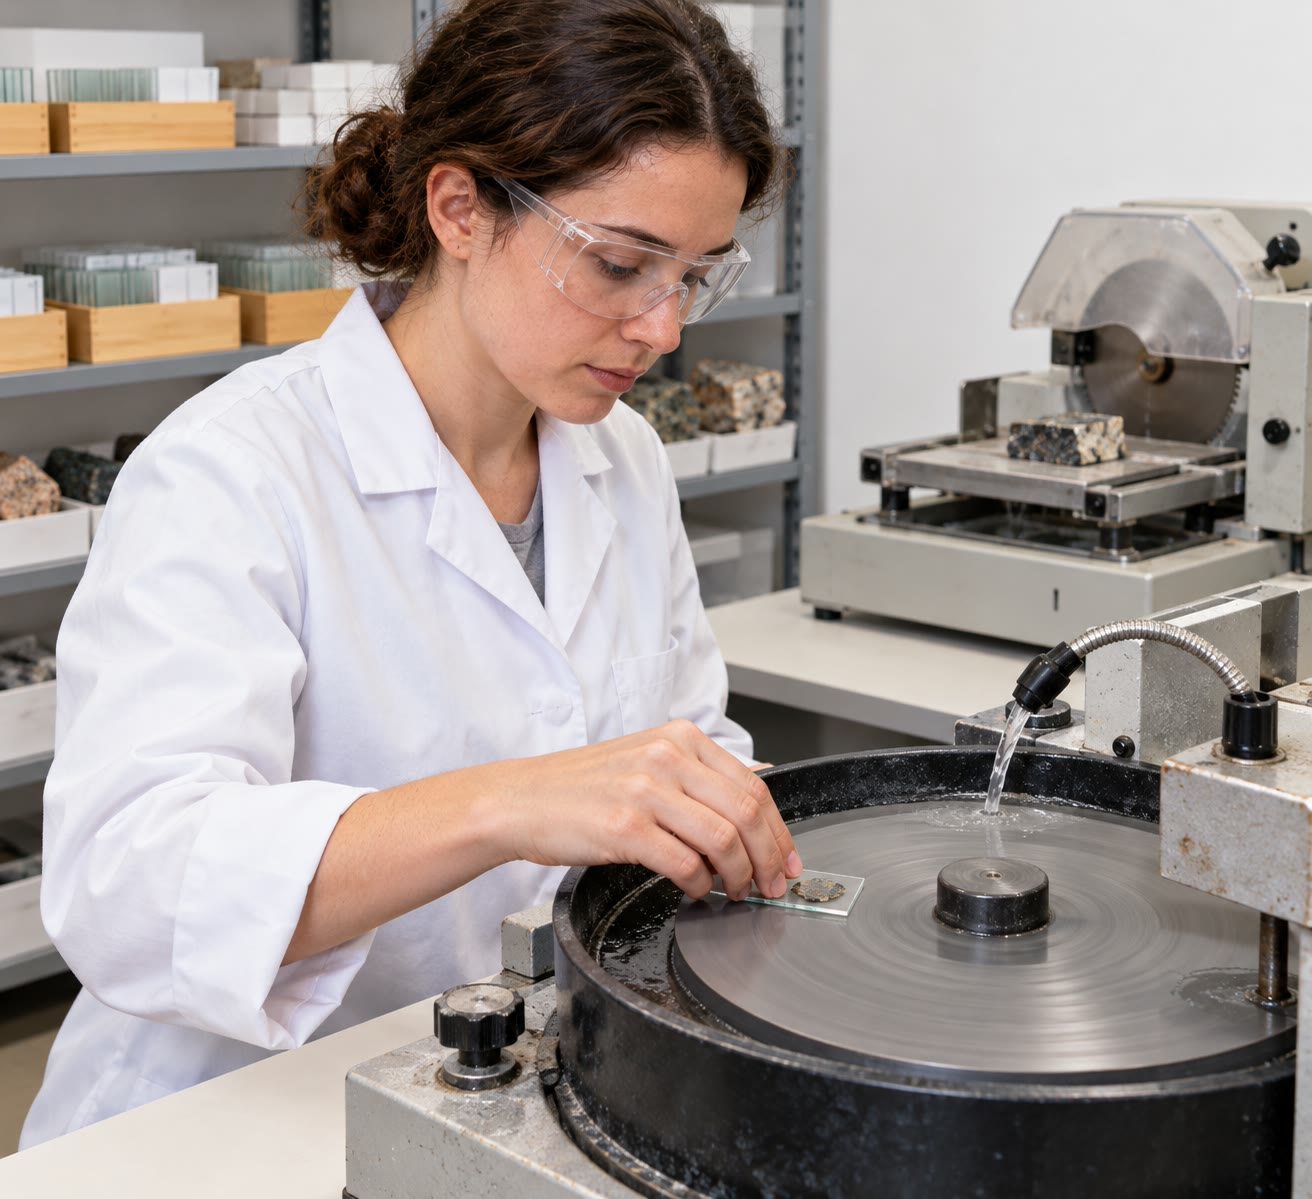
\includegraphics[width=\linewidth]{images/book3/ai/b1-thin-section-lab.jpg}
\end{minipage}
\end{inthelab}

Het slijpplaatje wordt bestudeerd met een microscoop die twee polariserende filters heeft. Lineaire polarisatie is het onderwerp
van de natuurkunde: hier volstaat het dat een polariserend filter alleen licht doorlaat dat in één \omterm{def:b1:field-lab-methods-1:trend-plunge}{richting} trilt, en dat twee
filters onder rechte hoeken niets doorlaten.

\begin{definition}[Polariserende microscoop, vlakgepolariseerd licht, gekruiste polarisatoren]\label{def:b1:field-lab-methods-1:microscope}
Een \emph{polariserende microscoop}\index{polariserende microscoop} is een doorlichtmicroscoop met een polariserend filter
(de polarisator) onder een tafel die over \ang{360} draait langs een geijkte schaal, en een tweede polariserend filter
(de analysator) tussen de objectieflens en het oculair, dat in of uit de lichtweg kan worden bewogen, met zijn trillingsrichting
onder rechte hoeken op die van de polarisator. Met de analysator eruit wordt het preparaat gezien in
\emph{vlakgepolariseerd licht}\index{vlakgepolariseerd licht}; met de analysator erin wordt het gezien tussen
\emph{gekruiste polarisatoren}\index{gekruiste polarisatoren}.
\end{definition}

\begin{omfigure}
\begin{tikzpicture}[font=\scriptsize, x=1cm, y=0.62cm]
\def\comp#1#2#3{\draw[fill=#3] (-1.1,#1-0.18) rectangle (1.1,#1+0.18); \node[right] at (1.3,#1) {#2};}
\draw[omThm!60, line width=3pt, -{Stealth[length=3mm]}] (0,0.3) -- (0,10.6);
\draw[fill=yellow!40] (0,0) circle (0.3); \node[right] at (1.3,0) {lamp};
\comp{1.3}{polarisator: laat één trillingsrichting door}{omDef!25}
\draw[omDef, thick, <->] (-0.5,1.3) -- (0.5,1.3);
\draw[fill=white] (-1.0,2.3) .. controls (0,2.75) .. (1.0,2.3) .. controls (0,1.85) .. (-1.0,2.3);
\node[right] at (1.3,2.3) {condensor};
\draw[fill=black!70] (-1.6,3.4) rectangle (1.6,3.55);
\draw[fill=icsJurassic!40] (-0.5,3.55) rectangle (0.5,3.65);
\node[right] at (1.7,3.48) {draaibare tafel, in graden verdeeld, met de slijpplaat};
\draw[fill=white] (-0.45,4.5) rectangle (0.45,5.4); \node[right] at (1.3,4.95) {objectief};
\comp{6.2}{sleuf voor accessoires}{black!10}
\comp{7.2}{analysator: erin (gekruiste polarisatoren) of eruit (vlakgepolariseerd licht)}{omDef!25}
\draw[omDef, thick, <->] (0,6.85) -- (0,7.55);
\comp{8.2}{Bertrandlens (optioneel)}{black!5}
\draw[fill=white] (-0.35,9.1) rectangle (0.35,10.0); \node[right] at (1.3,9.55) {oculair met draadkruis};
\end{tikzpicture}

{\small De lichtweg van een \omterm{def:b1:field-lab-methods-1:microscope}{polariserende microscoop} (schematisch, van onder naar boven). De polarisator en de analysator trillen
onder rechte hoeken (dubbele pijlen); met niets ertussen geven \omterm{def:b1:field-lab-methods-1:microscope}{gekruiste polarisatoren} een zwart veld.}
\end{omfigure}

Tussen \omterm{def:b1:field-lab-methods-1:microscope}{gekruiste polarisatoren} blijven het glas van het plaatje, de epoxy en elk isotroop mineraal (een mineraal waarvan de optische
eigenschappen in elke \omterm{def:b1:field-lab-methods-1:trend-plunge}{richting} gelijk zijn, zoals kubische kristallen) zwart, wat de draaiing van de tafel ook is. De meeste mineralen
zijn niet isotroop: zij veranderen de polarisatie van het licht dat erdoorheen gaat, en verschijnen in interferentiekleuren die
veranderen wanneer de tafel draait en die viermaal in een volledige omwenteling verdwijnen. Waarom zij dat doen, en hoe de kleuren en de
hoeken een mineraal identificeren, is het onderwerp van \cref{ch:b1:optical-mineralogy}.
Mineralen in een \omterm{def:b1:field-lab-methods-1:thin-section}{slijpplaat} worden meestal onderzocht bij vergrotingen van ongeveer
$16\times$ tot $400\times$.
% ledger: jaic:magnification

\begin{omfigure}
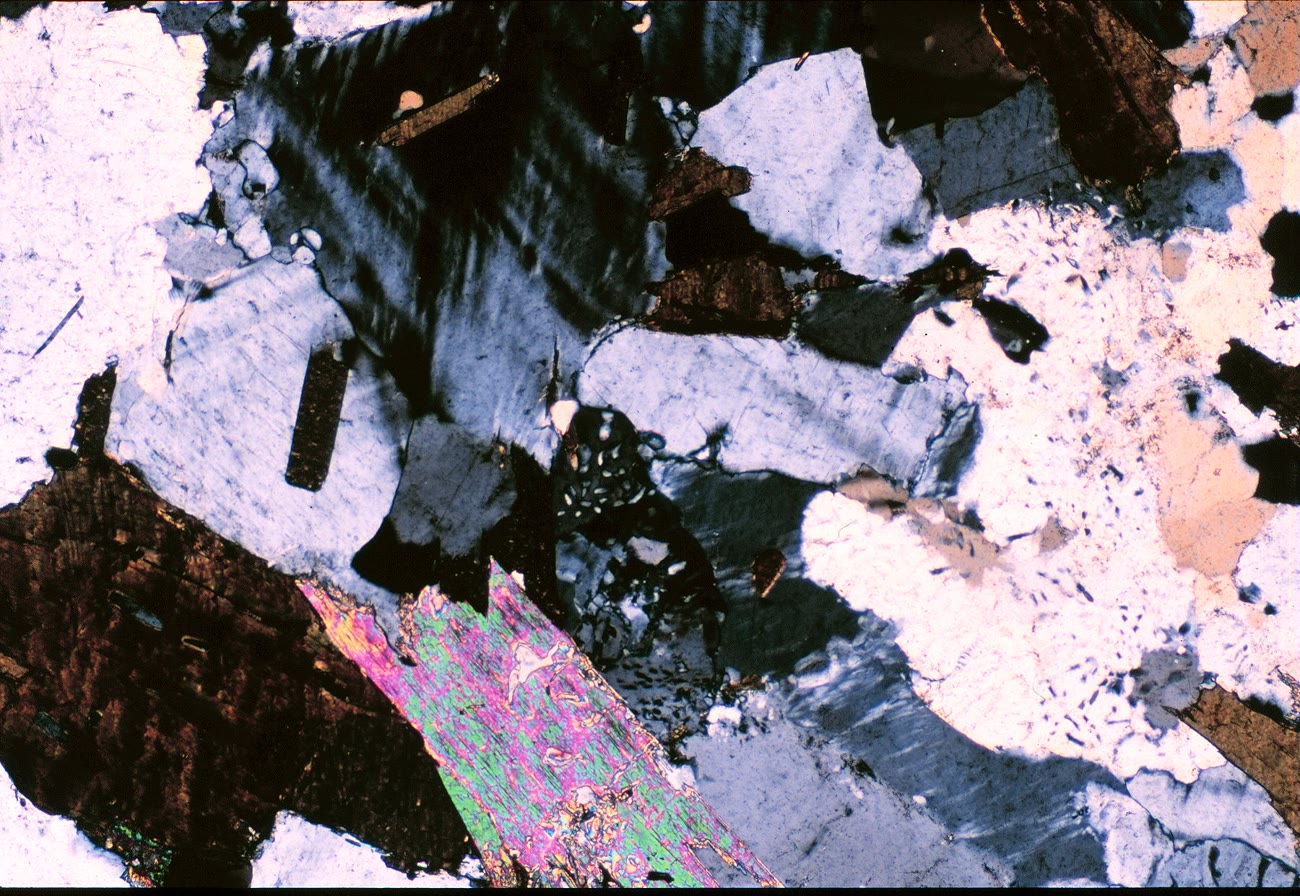
\includegraphics[width=0.55\linewidth]{images/book3/b1-granite-thin-section-xpl.jpg}
% ledger: commons:granite-xpl

{\small Een graniet in \omterm{def:b1:field-lab-methods-1:thin-section}{slijpplaat} tussen \omterm{def:b1:field-lab-methods-1:microscope}{gekruiste polarisatoren}. Biotiet is bruin, muscoviet toont heldere roze en groene
interferentiekleuren, plagioklaas is gestreept door zijn tweelingvorming, en kwarts is wit tot grijs. Foto Darla Sondrol, CC0
(Wikimedia Commons).}
\end{omfigure}

\begin{safety}
Veld- en laboratoriumwerk worden veilig gemaakt door professionele regels, niet door toeval. In het veld werken geologen in paren
of laten zij een schriftelijk plan van hun route en hun terugkeertijd achter; zij dragen weersvoorspellingen, kaarten en eerstehulp
bij zich, blijven weg van de voet en de rand van rotswanden en steengroefwanden, en dragen een helm en oogbescherming waar gesteente
kan vallen of splinteren; werk op actieve terreinen volgt de regels van de exploitant. In het laboratorium draaien zagen en schijven
achter beschermkappen, met water om stof te beperken; harsen en zuren worden met handschoenen en veiligheidsbril onder afzuiging
gehanteerd, en elke chemische stof heeft een veiligheidsinformatieblad. Geen van deze activiteiten is alleen voor een lezer van dit
boek bedoeld: het hoofdstuk beschrijft professionele praktijk.
\end{safety}

\section{Oefeningen}

\begin{exercise}[$\star$]\label{exo:b1:field-lab-methods-1:1}
Een satellietontvanger geeft posities binnen ongeveer \qty{4.9}{m}. Hoe groot is dat op een kaart van
1:10\,000? Op 1:25\,000?
\end{exercise}

\begin{exercise}[$\star$]\label{exo:b1:field-lab-methods-1:2}
Een kompas zonder declinatie-instelling leest de \omterm{def:b1:geological-maps:attitude}{hellingrichting} \ang{052} op een laag af. Geef de
geografische \omterm{def:b1:geological-maps:attitude}{hellingrichting} als de aflezing in Reykjavik op 1 januari 2026 is gedaan, en daarna in
Wellington op dezelfde dag (gedateerd kader).
\end{exercise}

\begin{exercise}[$\star$]\label{exo:b1:field-lab-methods-1:3}
Een \omterm{def:b1:geological-maps:fold}{plooias} duikt \ang{20} naar \ang{015}. Schrijf zijn oriëntatie zoals in de tekst en geef zijn neerwaartse
eenheidsvector in oost-, noord- en opwaartse componenten.
\end{exercise}

\begin{exercise}[$\star$]\label{exo:b1:field-lab-methods-1:4}
Drie aflezingen van een verticale spleet geven de \omterm{def:b1:spherical-astronomy:horizontal}{azimuten} van haar normaal \ang{350}, \ang{358} en \ang{006}.
Bereken hun rekenkundig gemiddelde, en daarna het \omterm{def:b1:spherical-astronomy:horizontal}{azimut} van de som van de drie horizontale eenheidsvectoren.
Welk gemiddelde is juist?
\end{exercise}

\begin{exercise}[$\star\star$]\label{exo:b1:field-lab-methods-1:5}
Vijf aflezingen van de helling van één laag zijn \ang{34}, \ang{37}, \ang{35}, \ang{33} en \ang{36}. Bereken hun
gemiddelde, hun standaardafwijking en de standaardfout van het gemiddelde.
\end{exercise}

\begin{exercise}[$\star\star$]\label{exo:b1:field-lab-methods-1:6}
Een geoloog middelt één aflezing op elke poot van een symmetrische \omterm{def:b1:geological-maps:fold}{plooi}: $090/30$ en $270/30$. Bereken het
vectorgemiddelde en $\bar R$. Wat is er misgegaan?
\end{exercise}

\begin{exercise}[$\star\star$]\label{exo:b1:field-lab-methods-1:7}
Krassen op een gelaagdheidsvlak met oriëntatie $080/12$ hebben de \omterm{def:b1:field-lab-methods-1:trend-plunge}{richting} \ang{120}. Wat is hun \omterm{def:b1:field-lab-methods-1:trend-plunge}{duik}? Wat zou die
zijn voor de \omterm{def:b1:field-lab-methods-1:trend-plunge}{richting} \ang{170}?
\end{exercise}

\begin{exercise}[$\star\star$]\label{exo:b1:field-lab-methods-1:8}
In Edinburgh is de magnetische declinatie op 1 januari 2026 \ang{-0.47} en verandert zij met \ang{+0.20} per jaar.
Wanneer bereikt zij, als de verandering gelijkmatig blijft, nul, en hoe groot is zij op 1 januari 2030?
\end{exercise}

\begin{exercise}[$\star\star$]\label{exo:b1:field-lab-methods-1:9}
Drie aflezingen van één laag zijn $080/10$, $080/12$ en $080/14$. Toon aan dat hun vectorgemiddelde $080/12$ is,
bereken $\bar R$ en de schatting $\sqrt{2(1 - \bar R)}$ van $\theta_{\text{rms}}$, en vergelijk met de exacte
kwadratisch gemiddelde hoek.
\end{exercise}

\begin{exercise}[$\star\star\star$]\label{exo:b1:field-lab-methods-1:10}
Een \omterm{def:b1:field-lab-methods-1:thin-section}{dunne slijpplaat} snijdt een bolvormige korrel met straal $r$ op een afstand $h$ van zijn middelpunt, met $h$
overal tussen 0 en $r$ even waarschijnlijk. Toon aan dat de gemiddelde straal van de cirkel die in de doorsnede
wordt gezien $\pi r/4$ is. Kwartskorrels van \qty{0.50}{mm} doorsnede lijken in een \omterm{def:b1:field-lab-methods-1:thin-section}{slijpplaat} gemiddeld hoe groot?
\end{exercise}

\begin{exercise}[$\star\star\star$]\label{exo:b1:field-lab-methods-1:11}
Toon aan dat als elke \omterm{def:b1:geological-maps:attitude}{hellingrichting} van een reeks aflezingen met dezelfde hoek $D$ wordt verhoogd, de
\omterm{def:b1:geological-maps:attitude}{hellingrichting} van hun vectorgemiddelde met $D$ toeneemt en dat de helling niet verandert. Waarom is dat van
belang voor de declinatiecorrectie?
\end{exercise}

\begin{exercise}[$\star\star\star$]\label{exo:b1:field-lab-methods-1:12}
Op een laag van \ang{12} varieert de normaal van één aflezing met een standaardafwijking van \ang{2} in elk van twee
loodrechte \omterm{def:b1:field-lab-methods-1:trend-plunge}{richtingen}: langs de lijn van de steilste helling, wat de helling verandert, en er dwars op, wat de
\omterm{def:b1:geological-maps:attitude}{hellingrichting} verandert. Hoeveel aflezingen zijn nodig voor een standaardfout van \ang{0.5} op de gemiddelde helling?
Van \ang{1} op de gemiddelde \omterm{def:b1:geological-maps:attitude}{hellingrichting}?
\end{exercise}

\section{Probleem: Een veldseizoen op de oostflank van Varden}

\begin{problem}[{Weekendprobleem --- twaalf kompasaflezingen middelen, hun spreiding meten, ze corrigeren en
ze vergelijken met de boringen}]
\label{pb:b1:field-lab-methods-1:1}
% readings: figdata/bachelor-1/attitude_stats.py (part normals); values: calc/ch06.py
Een geoloog mat de gelaagdheid van de oostflank van de \omterm{def:b1:geological-maps:fold}{antiklinaal} van Varden op twaalf standplaatsen, met een
kompas dat voor de declinatie was ingesteld, afgerond op de graad. De tabel geeft elke aflezing
(\omterm{def:b1:geological-maps:attitude}{hellingrichting}/helling) en de componenten van haar opwaartse eenheidsnormaal $\vec n = (n_E, n_N, n_U)$, afgerond op
vier decimalen.
\begin{center}
\small
\begin{tabular}{rcccc@{\qquad}rcccc}
\hline
 & aflezing & $n_E$ & $n_N$ & $n_U$ & & aflezing & $n_E$ & $n_N$ & $n_U$ \\
\hline
1 & $076/11$ & 0.1851 & 0.0462 & 0.9816 & 7 & $083/11$ & 0.1894 & 0.0233 & 0.9816 \\
2 & $081/13$ & 0.2222 & 0.0352 & 0.9744 & 8 & $083/12$ & 0.2064 & 0.0253 & 0.9781 \\
3 & $078/16$ & 0.2696 & 0.0573 & 0.9613 & 9 & $085/12$ & 0.2071 & 0.0181 & 0.9781 \\
4 & $081/11$ & 0.1885 & 0.0298 & 0.9816 & 10 & $078/11$ & 0.1866 & 0.0397 & 0.9816 \\
5 & $076/10$ & 0.1685 & 0.0420 & 0.9848 & 11 & $081/13$ & & & \\
6 & $083/14$ & 0.2401 & 0.0295 & 0.9703 & 12 & $082/11$ & & & \\
\hline
\end{tabular}
\end{center}

\medskip
\noindent\textbf{Deel I --- Het gemiddelde van de oriëntatie.}
\begin{enumerate}
  \item Bereken de rekenkundige gemiddelden van de twaalf \omterm{def:b1:geological-maps:attitude}{hellingrichtingen} en van de twaalf hellingen.
  \item Geef een voorbeeld van twee aflezingen waarvoor het rekenkundig gemiddelde van de \omterm{def:b1:geological-maps:attitude}{hellingrichtingen}
        absurd is, en zeg waarom het hier veilig is.
  \item Toon aan dat $\vec n = (\sin\delta\sin\alpha, \sin\delta\cos\alpha,
        \cos\delta)$ een eenheidsvector is die loodrecht staat op de hellingslijn en op
        de strijklijn van het vlak $\alpha/\delta$.
  \item Vul de tabel aan voor de aflezingen 11 en 12.
  \item Bereken de resultante $\vec S$ van de twaalf normalen.
  \item Bereken $\|\vec S\|$ en de gemiddelde resultantelengte $\bar R$.
  \item Leid het vectorgemiddelde af: zijn \omterm{def:b1:geological-maps:attitude}{hellingrichting} en zijn helling.
\end{enumerate}

\medskip
\noindent\textbf{Deel II --- De spreiding.}
\begin{enumerate}[resume]
  \item Bereken de steekproefstandaardafwijkingen van de \omterm{def:b1:geological-maps:attitude}{hellingrichtingen} en van de hellingen.
  \item Gebruik \cref{prop:b1:field-lab-methods-1:vector-mean} om de kwadratisch gemiddelde hoek
        $\theta_{\text{rms}}$ tussen de aflezingen en hun gemiddelde te schatten, in graden.
  \item Voorspel $\theta_{\text{rms}}$ uit de twee standaardafwijkingen van vraag 8 en de foutformule van het
        hoofdstuk, en vergelijk.
  \item Welke van de twee standaardafwijkingen draagt het meest bij aan $\theta_{\text{rms}}$, en waarom?
  \item Bereken de standaardfouten van de gemiddelde helling en van de gemiddelde \omterm{def:b1:geological-maps:attitude}{hellingrichting}.
  \item Is de spreiding van de \omterm{def:b1:geological-maps:attitude}{hellingrichtingen}, \ang{2.9}, een teken van onzorgvuldig meten? Leg uit.
\end{enumerate}

\medskip
\noindent\textbf{Deel III --- De declinatie.}
\begin{enumerate}[resume]
  \item Een tweede geoloog vergat de declinatie in te stellen. Haar twaalf aflezingen hebben het vectorgemiddelde
        $083.1/12.1$ in magnetische \omterm{def:b1:spherical-astronomy:horizontal}{azimuten}. Stel dat de magnetische declinatie in de Varden Hills dat jaar
        \ang{2.5} west is. Wat is haar gemiddelde in geografische \omterm{def:b1:spherical-astronomy:horizontal}{azimuten}?
  \item Waarom is haar gemiddelde helling zonder correctie juist?
  \item Had zij elke aflezing kunnen corrigeren vóór het middelen, in plaats van het gemiddelde? Verandert het
        antwoord (\cref{exo:b1:field-lab-methods-1:11})?
  \item Tien jaar later hergebruikt een student haar declinatie-instelling terwijl de declinatie met \ang{0.2} per
        jaar is veranderd. Hoe groot is de fout, vergeleken met de standaardfout van vraag 12?
  \item Geef de \omterm{def:b1:geological-maps:attitude}{strijk} van het gemiddelde van de eerste geoloog volgens de rechterhandregel.
\end{enumerate}

\medskip
\noindent\textbf{Deel IV --- Kompas en boringen.}
\begin{enumerate}[resume]
  \item Uit drie boringen vond \cref{ch:b1:geological-maps} de oriëntatie $080.6/12.2$ voor de basis van de kalksteen.
        Vergelijk die hoek voor hoek met het vectorgemiddelde van vraag 7.
  \item Bereken de hoek tussen de twee normalen.
  \item De standaardfout van de gemiddelde \omterm{def:b1:field-lab-methods-1:trend-plunge}{richting} is ongeveer $\theta_{\text{rms}}/\sqrt N$. Is het verschil van
        vraag 20 significant?
  \item Hoeveel aflezingen zouden die standaardfout halveren?
  \item Noem twee fouten die geen aantal aflezingen zou verkleinen.
  \item Geef de \omterm{def:b1:field-lab-methods-1:mean-orientation}{gemiddelde oriëntatie} van de oostflank uit de twaalf aflezingen, in de vorm \omterm{def:b1:geological-maps:attitude}{hellingrichting}/helling,
        afgerond op de graad.
\end{enumerate}
\end{problem}
